\documentclass[letterpaper, 10 pt, conference]{ieeeconf}  % Comment this line out if you need a4paper

%\documentclass[a4paper, 10pt, conference]{ieeeconf}      % Use this line for a4 paper

\IEEEoverridecommandlockouts                              % This command is only needed if 
                                                          % you want to use the \thanks command

\overrideIEEEmargins                                      % Needed to meet printer requirements.

% The following packages can be found on http:\\www.ctan.org
\usepackage{graphics} % for pdf, bitmapped graphics files
%\usepackage{graphicx}
\usepackage[dvipdfmx]{graphicx}
\usepackage[dvipdfmx]{color}
\usepackage{epsfig} % for postscript graphics files
\usepackage{mathptmx} % assumes new font selection scheme installed
\usepackage{times} % assumes new font selection scheme installed
\usepackage{amsmath} % assumes amsmath package installed
\usepackage{amssymb}  % assumes amsmath package installed
\usepackage{multicol}
\usepackage{multirow}
\usepackage{url}
\usepackage{caption}
\usepackage[ruled,vlined]{algorithm2e}
%\include{pythonlisting}
\usepackage{algpseudocode}
\usepackage[dvipsnames]{xcolor}
\usepackage{cite}

\setlength\textfloatsep{5pt}

\title{\LARGE \bf
Time-Based Current Source (TBCS): A Highly-Digital PVT Adaptive Current Generator for Switched Capacitor Circuits
}

\author{Kentaro Yoshioka% <-this % stops a space
%\thanks{*This work was not supported by any organization}% <-this % stops a space
\thanks{
        {\tt\small yoshioka@elec.keio.ac.jp}}
}

\begin{document}

\maketitle
\thispagestyle{empty}
\pagestyle{empty}

%%%%%%%%%%%%%%%%%%%%%%%%%%%%%%%%%%%%%%%%%%%%%%%%%%%%%%%%%%%%%%%%%%%%%%%%%%%%%%%%
\begin{abstract}
VCO比較機ではdeadzone特性を使用することで自動的にIRN性能を入力に適した値に設定する。
The proposed adaptive time-domain (ATD) comparator automatically adjusts its input-referred noise performance according to the intermediate residual input level (?Vin) during conversion. Considering

入力に応じたオンデマンドのノイズと消費電力の比較器を提供。


\end{abstract}

%%%%%%%%%%%%%%%%%%%%%%%%%%%%%%%%%%%%%%%%%%%%%%%%%%%%%%%%%%%%%%%%%%%%%%%%%%%%%%%%
\section{Introduction}
スイッチドキャパシタ回路はパイプライン ADC、Pipeline-SAR ADCといった高精度・高速ADCの根幹を担う回路ブロックであり、5G、beyond 5Gといった先端通信回路を構成する\cite{ali201414, ali202012, lagos2018single, hung2020calibration}。基準電流源はこのようなスイッチドキャパシタ回路におけるオペアンプ特性を決定づける重要な回路である。特に高速なスイッチドキャパシタ回路であるとオペアンプの速度(ユニティゲイン)は重要な設計パラメータであり、注意深く設計する必要がある。しかしオペアンプ自体の設計に加え基準電流源のPVTばらつき性能は大きくスイッチドキャパシタ速度に寄与する一方であまり文献で注目されてはいなかった。

基準電流源は主にbeta-multiplierか電圧電流変換と2種類の設計アプローチがある。self-bias方式で電流を生成するbeta-multiplierは抵抗とトランジスタの温度特性が相補的であることを利用し、温度依存性をキャンセルする\cite{azcona2014precision, osipov2016temperature}。また電圧電流変換アプローチはPVTばらつきの影響が少ないBGR電圧源で生成した基準電圧を元に抵抗を用いて電圧ー電流変換を行う\cite{banba1999cmos, ueno2009300}。一方で両方の方式でも生成電流は抵抗値に応じて決定される。一般的な電流源は数10uAオーダであり、数10kオームのポリ抵抗阻止が用いられる。しかしこれらの抵抗値は量産時に製造ばらつきによって抵抗値は±50\%ほどばらついてしまい、そのドリフトは生成電流に直接現れる。

そのためこのような抵抗ばらつきは出荷テスト時にキャリブレーションするか設計マージンとして許容するのが一般的である。しかし前者は高コストなアナログテスト工数の増加を招き、後者はオペアンプのオーバーデザインにより消費電力、面積、歩留まりを悪化させる。電流源に用いる抵抗をトランジスタで置き換える研究も存在するが\cite{hirose2010nano, osaki20131, choi201423pw}、マッチングやアナログ特性が重要であるため回路面積は大きいためCMOSスケーリングに応じたコスト削減が難し。

本論文では低コストかつプロセススケーラブルな電流源を実現するために時間情報を基準とする電流源(TBCS)を提案する\cite{yoshioka201728}。具体的にはcurrent-starved inverterをADCのサンプルクロックでロックするDLL(delay-locked-loop)を構築し、セトリングした電流値を直接基準電流として用いる。current-starved inverterの遅延は電流と負荷容量で決定されるため、遅延を一定値にロックすることで一定電流を供給するレファレンスを構築できる。重要なことにTBCSはPVTに対し*適応的*な電流生成を行う。負荷容量が増加するようなPVT条件の場合、本電流源は遅延を一定に保つため生成電流は増加する。これは増加したオペアンプに対しても増大した負荷容量の影響をキャンセルし速度一定に保つ効果がある。TBCSはほぼインバータセルとデジタル回路で構成でき、高いCMOS親和性を持ちプロセススケーラビリティは高い。試作回路は28nmCMOSにおいて面積はたったの800um2でありながらPVTばらつきに対し頑強であった。

Ref.\cite{yoshioka201728}に対し追加して本論文はTBCSについてextensiveな課題探索、解析を追加する。具体的には以下のような貢献をする。

- TBCSの原理、回路インプリについて深い議論を行うのに加え詳細シミュレーションによりTBCSをオペアンプとスイッチドキャパシタ回路に組み込んだ際の特性を報告し、PVT追従性を明らかにする

本論文の構成について述べる。2章では従来研究とそれらの課題について述べる。3章ではTBCSの原理について説明し、4章ではTBCSの回路インプリについて議論し最後に5章でシミュレーション結果と解析について報告する。

%\section{Comparison of systematic comparator power consumption}
\section{Related researches}
\begin{figure}[!]
\centering
 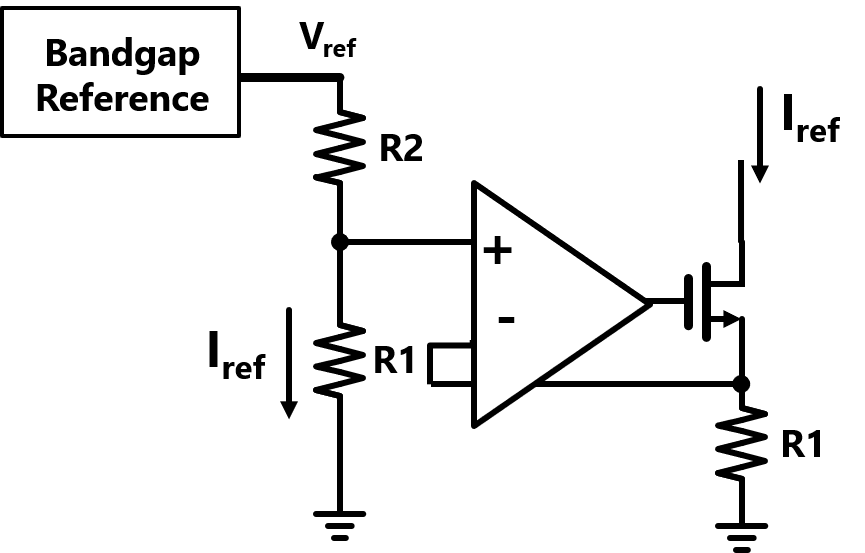
\includegraphics[width=0.5\textwidth]{figs/fig1.png}
  \caption{(a) 
}
\label{fig2}
\end{figure}

\begin{figure*}[!]
\centering
 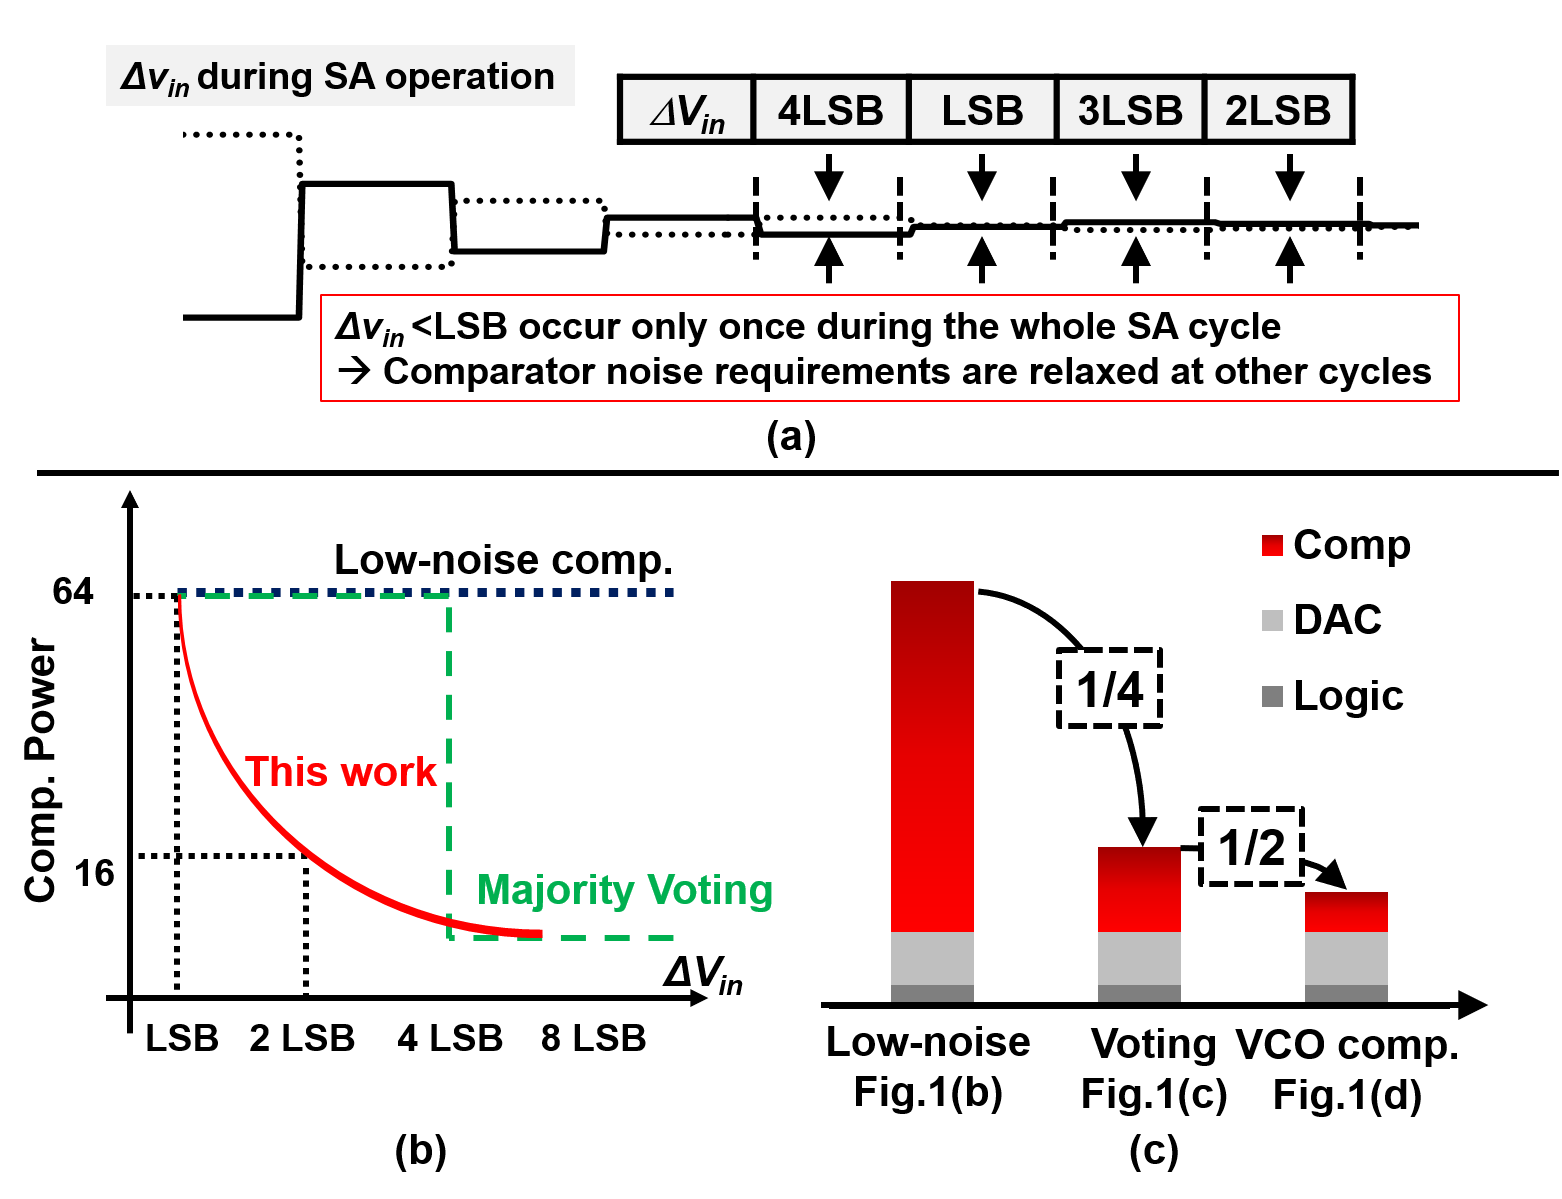
\includegraphics[width=0.9\textwidth]{figs/fig2.png}
  \caption{VCO comparator block diagram and its timing chart. (a)-(c) shows the VCO waveform when $\Delta V_{in}$=11-bit LSB and 13-bit LSB are given, respectively.}
  \label{fig2}
\end{figure*}
\textbf{バンドギャップレファレンス} 広く電流源として使用されるバンドギャップ・リファレンスを図2に示す。バンドギャップ・リファレンス回路は参照電圧VREFを生成し、
\begin{eqnarray}
    \centering
    I_{ref} = \frac{V_{ref}}{R_1 + R_2}
    \label{sar13b}
\end{eqnarray}
となる基準電流(IREF)を生成する。バンドギャップ・リファレンスは環境変動(温度、トランジスタしきい値、電源電圧等。以下PVTばらつきと呼ぶ)の影響を受けずに一定の電位を生成することができる。一方で抵抗値R1及びR2は製造ばらつきの影響を大きく受け、抵抗値はポリ抵抗であった場合最大で$\pm 50\%$程度ばらつく。そのため$I_{ref}$=20uAをターゲットとした場合、max-min電流値はそれぞれ40uA、13uAと非常に大きな幅を持つ。このようなばらつきはオペアンプの設計マージンを拡大させ消費電力を増加する。

\textbf{適応的電流源技術} PVTに適応して動作する電流源技術はミックスドシグナル製品開発上重要であり、多くの研究がなされている。Ref.\cite{chuanyang,ron}はレプリカのアンプとチャージ用容量を用意し、オペアンプのスルーレートを直接観測することで所定のスルーレートを実現するよう電流にフィードバックをかけPVTに追従する適応的電流源を実現する。
一方でレプリカのオペアンプが必要となるため消費電力、面積のオーバーヘッドは大きい。一方でTBCSはレプリカアンプを用意することなく、ほぼデジタル素子を用いてPVTロバストな電流源を実現可能でオーバーヘッドは小さい。

\textbf{時間情報を用いたアナログ回路キャリブレーション技術} Ref.\cite{zhu}は基準クロックの時間情報を用いてアナログ回路素子をキャリブレーションする。具体的には電源電圧をDLLを用いて一定遅延になるよう制御し、基本的なアイデアはTBCSと同様である。
またDLLを用いて非同期SARクロックの遅延を制御し、DACセトリング時間をキャリブレーションする研究も存在する\cite{kapusta201314b,tompson}。
一方でオペアンプに用いる基準電流源のばらつきを時間情報を用いて抑え込む研究は著者の知る限りTBCSが初である。

\section{Time based current source}
\subsection{TBCS fundamentals}

図\ref{fig2}にTBCSの簡略化した回路ブロック図を示す。TBCSの必要な入力は所定周波数のクロック$CLK$(ADCのサンプルクロック等)のみであり、Delay-Locked-Loop回路(DLL)と構成要素や動作は近い。基準電流源はレファレンス電流($I_{ref}$)を作り出し、オペアンプといったコア回路に与える。またTBCSではcurrent-starved-delayline(CSD)にも$I_{ref}$を与え、CSDは$CLK$に対し遅延を加えた$CLK_D$を出力する。CSDのステージ数を$N$としステージ遅延を$t_{DL}$とした場合、$CLK_D$は$CLK$に対し$Nt_{DL}$の遅延を生じる。ここで$I_{ref}$が大きいほど$t_{DL}$は小さくなりその逆も然りである。そして上述の遅延器出力とCLKの反転出力($CLK_B$)間で位相比較を行い、遅延($Nt_{DL}$)が$T_D$に漸近するよう基準電流源を制御し遅延を一定値に収束させる。

%TBCSは遅延器出力CLKDとCLKの反転出力(CLKB)間で位相比較を行い遅延(10*tDL)をCLKの半周期(TD)に漸近するよう電流を制御する。図 3右下にTBCSのプリンシパルとなる遅延器の電流-遅延特性を示す。

\begin{figure}[!]
\centering
 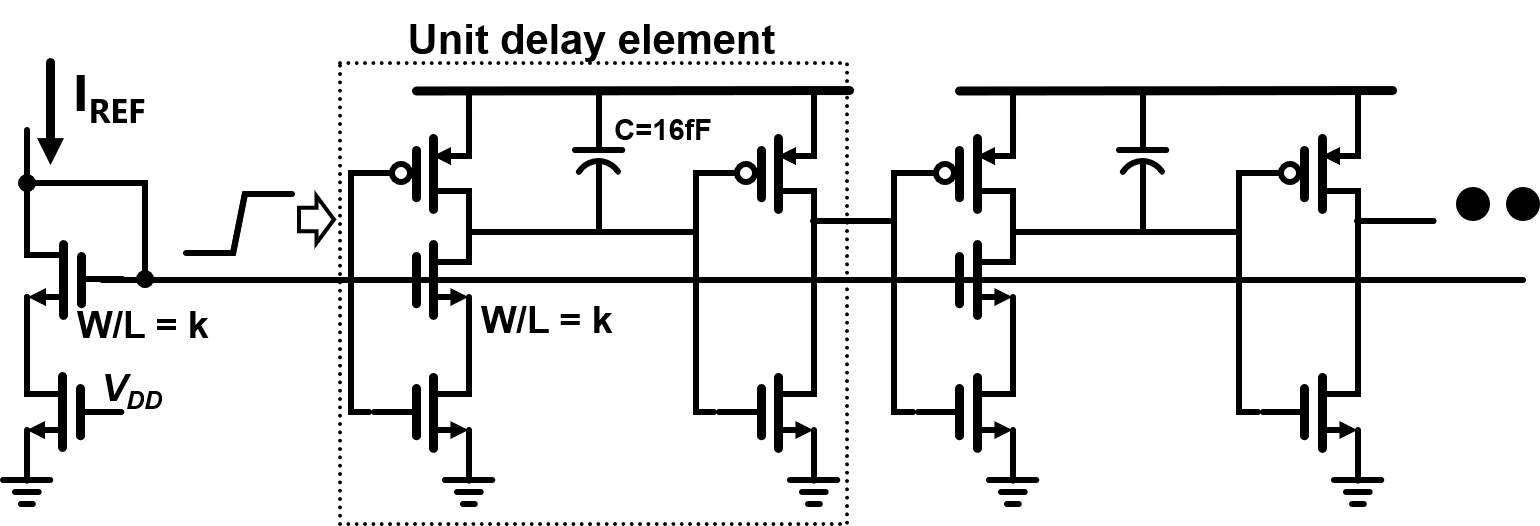
\includegraphics[width=0.5\textwidth]{figs/inv.png}
  \caption{(a) 
}
\label{inv}
\end{figure}

図\ref{inv}のような容量負荷を駆動するcurrent sturvedインバータ(CSI)\cite{mroszczyk2014tunable}とインバータを接続した遅延ステージ考える。大信号特性を元にCSIの遅延tDを考えると、次段インバータのオンしきい値をVthとし、インバータ遅延を$t_{inv}$とすると
\begin{eqnarray}
    \centering
    t_D = \frac{V_{th}C}{I_{Ref}}+t_{inv}
    \label{delay}
\end{eqnarray}

と表せる。CSIの電流源が三極管領域に入る頃には信号は次段へと伝搬しているため、そのような事象は解析にて無視できる。ここでtinvが前項より十分小さくインバータしきい値のばらつきも小さいと見なすと、tDはCとIrefによって決まると見なせる。そしてtDLを電流制御により一定遅延にロックするため、ロック時の電流はCのばらつきに応じた値が得られる。容量は電圧、温度といった環境変動に対して受ける影響は少なく、遅延tDLにロックした時の電流値は環境変動によらず一定なロバストな電流源となる。

上記の解析と式よりTBCSのばらつき要因には 1)負荷容量のばらつきと2)次段インバータ遅延、オンしきい値ばらつきがある。
次段インバータの影響はCSI遅延より1桁小さいため影響は少ない一方で、TBCSがロバストな電流源となるために負荷容量の絶対値ばらつきが小さいことが求められる。例えばmetal-insulator-metal(MIM)容量はミスマッチは少ないものの、絶対値ばらつきが大きいためTBCSにはそぐわない。一方で先端CMOSプロセスに主に使用される配線間寄生容量で作成するmetal-oxcide-metal(MOM)容量は絶対値ばらつきはMIM容量や抵抗素子よりも小さくTBCSに好適でありロバストな電流源を実現できる。またTBCSは容量ばらつきによって電流が変動してしまうが、次節にてこのようなTBCSのドリフトはオペアンプ特性を一定化するのに役立ちTBCSはPVTに適応的な性質を持つことを示す。


\subsection{PVTに適応した電流生成(オペアンプにとって好適なドリフトの議論)}
\begin{figure}[!]
\centering
 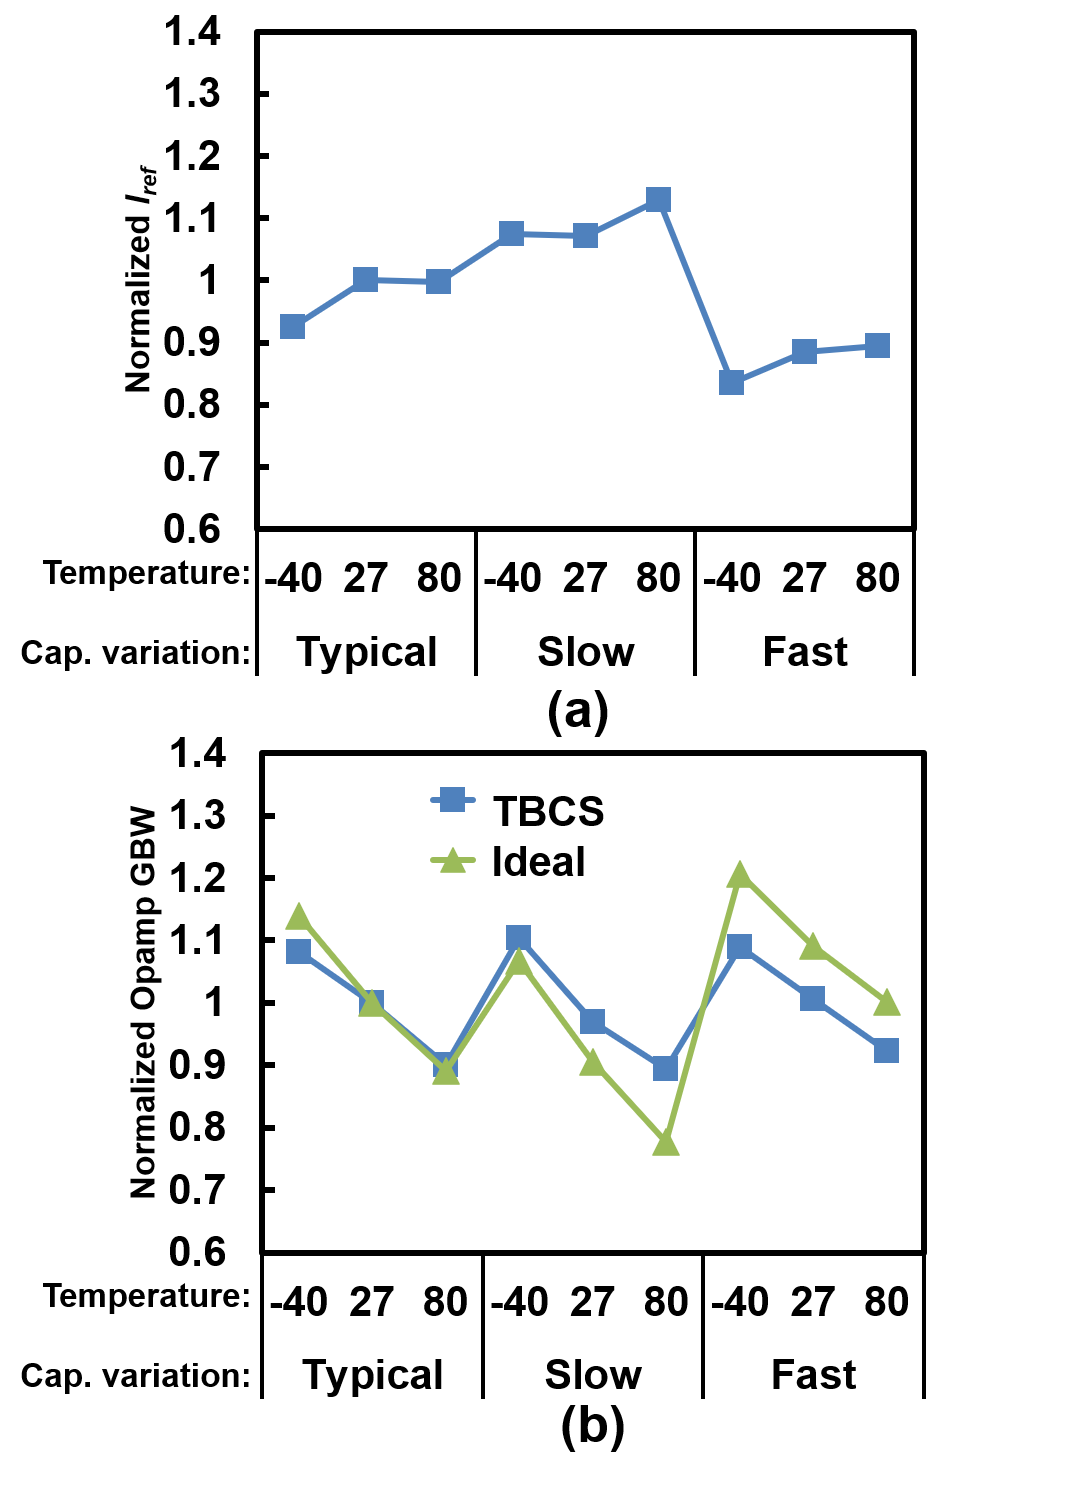
\includegraphics[width=0.5\textwidth]{figs/iref_var.png}
  \caption{(a) 
}
\label{cvar}
\end{figure}

TBCSはトランジスタや抵抗のPVTばらつきの影響は受けづらい反面、遅延を負荷容量の充電時間によって決めるため容量値ばらつきで生成電流が変動してしまう。しかし興味深いことにTBCSの容量ばらつきの電流変動はオペアンプのばらつき耐性を高めるよう作用しTBCSはPVTに適応した電流生成するといえる。
遅延の式eq.\ref{delay}よりCが増えるとTBCSの生成電流も増加し反対にCが減ると電流も減る。このような特性は一定の電流を生成する基準電流源という視点では望ましくない。一方でこのような容量ばらつきが起きる時、オペアンプの負荷容量も同様に増減する。負荷容量の増加によりオペアンプのGBWは悪化するものの、その減少分を補償するようにTBCSは電流を増やしGBWを一定に保つように働く。

図\ref{cvar}(a)に負荷容量が増大するPVT条件を作り出した際のTBCS生成電流をプロットし、図\ref{cvar}(b)に同ばらつき下におけるオペアンプGBWの変動をシミュレーションした結果を示す。Slowは負荷容量大、Fastは負荷容量小のばらつき条件をシミュレーションしている。SlowでTBCSの生成電流は10-15\%ほどは増加するが、この電流増加は負荷容量増大によって悪化したオペアンプのGBWを補償する。興味深いことにTBCSは一定電流を生成する理想電流源よりもオペアンプGBWをPVTを通し一定に保つ。
一般的な大量生産チップではオペアンプのGBWといった性能指標をワースト条件でも所定性能を満たすよう設計する。そのためワースト条件(Slow 80℃)におけるGBWが緩和されればされるほど、設計マージンを減らし消費電力を改善できる。図\ref{cvar}(b)では理想電流源に対してもTBCSを用いることでワースト条件のGBWを13\%改善することができ、設計マージン削減に大きく貢献する。


\section{Circuit Implementations}
\subsection{Control circuit and phase detector}
\begin{figure}[!]
\centering
 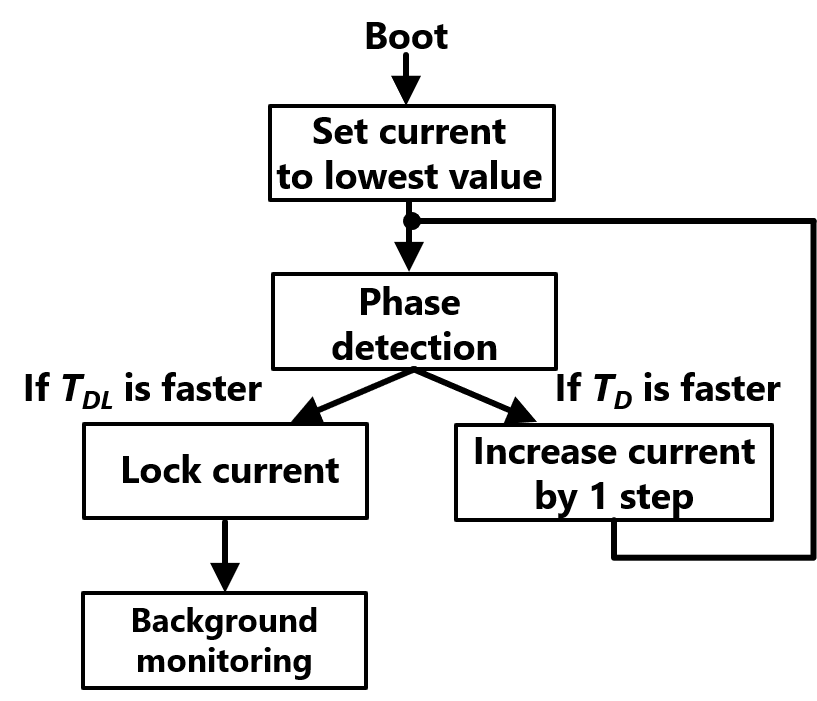
\includegraphics[width=0.5\textwidth]{figs/flowchart.png}
  \caption{(a) 
}
\label{flow}
\end{figure}
まずTBCSの基本的な制御について図\ref{flow}を用いて詳しく説明する。電流を制御するデジタルコードは電流が最低値になるような初期値を取り、そこから1コードずつ大きくしていくことで最適コードを探索する。最初期は電流が小さいため$t_{DL}$は長く、$T_D$に対し遅延は長くなる。もしTDの方が早いならば位相比較器は察知し、電流を1コード分増加させる(0→1)。この動作をTDLが早くなるまで繰り返す。

この制御方法は単純な反面、収束までの時間が最大$2^N$サイクルかかるという欠点がある(Nは電流源のbit数)。本電流源は5bitのため、最大32サイクル収束に必要である。例えば逐次比較のようなアルゴリズムであれば収束にかかるサイクル数は短くすることができるが、動作中に温度等がドリフトしてしまうとリアルタイムで追従できないといったトレードオフがある。

\begin{figure}[!]
\centering
 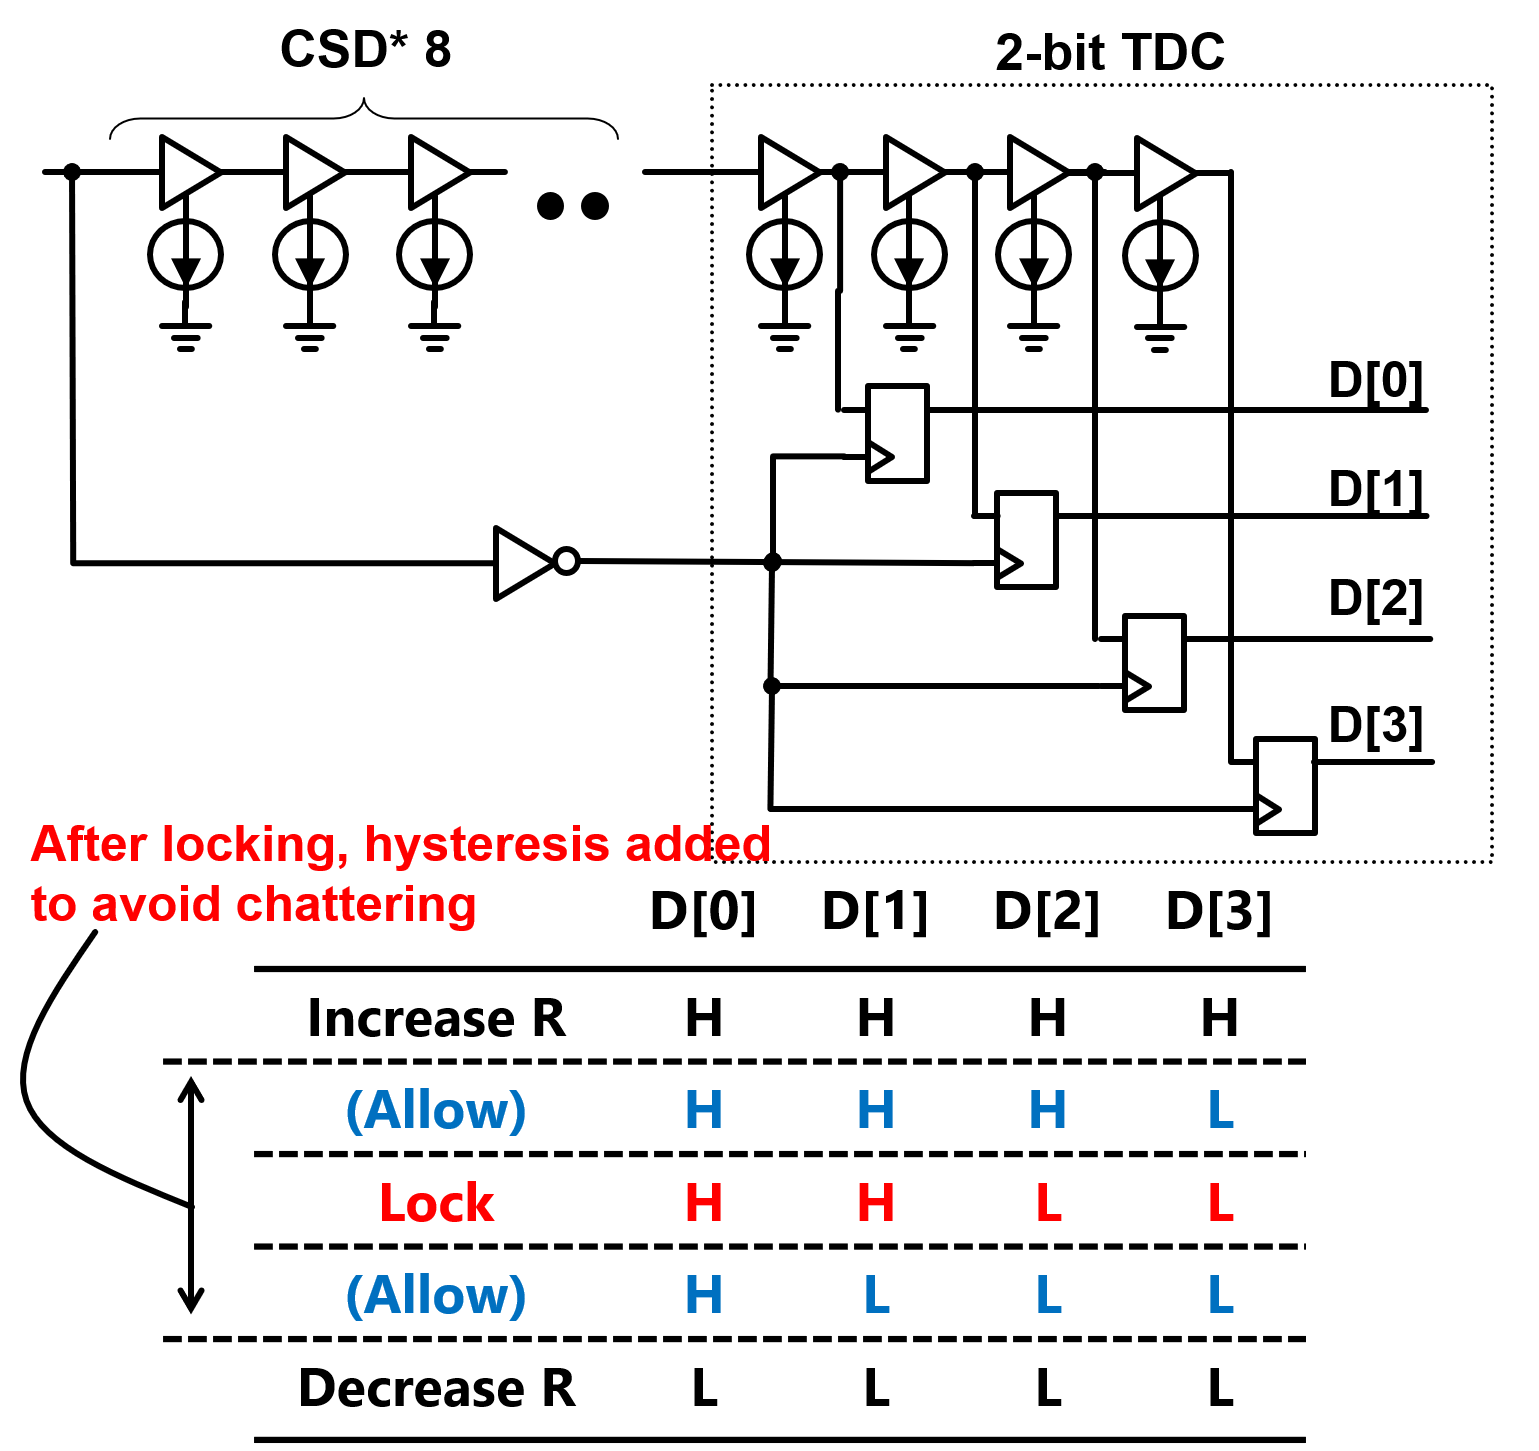
\includegraphics[width=0.5\textwidth]{figs/tdc.png}
  \caption{(a) 
}
\label{fig2}
\end{figure}

次に位相比較器の実装について述べる。本回路では位相比較器の設計を2bitにすることによって電流源がロックした後のチャタリングを防止しつつPVTドリフト追従機能をもたせる。1-bitのTDCは簡単にフリップフロップひとつで実現できるが、コードばたつき(チャタリング)の可能性がある。図 14にチャタリングが起きる例を示す。これは誇張して遅延変化を書いているが、最初の位相比較で遅延量を減らすように制御をした場合(コード14→15へ)、次の位相比較時には遅延がTDに対し小さくなってしまう可能性がある。この場合位相比較結果を受けて再び電流コードを減らす(15→14へ)ように制御を行うため堂々巡りになってしまう。結果毎サイクル電流値が変わることになってしまい、スイッチドキャパシタ回路において不要なスプリアスが発生する原因になりかねない。例えばcount-up制御のため、一度位相関係が逆転したら制御コードをロックするようにしてもよいが、それではPVTドリフトに対して追従することはできない。

TDLが早くなるとTBCSはロックし、その後は長期的なPVT変動に対応するバックグラウンドモニタリングを行う。図フローチャートではbang-bang制御であったが、バックグラウンドモニタ時にも同等制御を行うと常に電流のチャタリングが発生するため、TBCSでは2-bit TDCを用いてヒステリシスを備える。図にチャタリング対策を実施したディレイステージと2-bit TDCの回路図を示す。ロック前はbit D[1]のみモニタし電流値を制御し、ロック後は2-bit出力D[0:3]を用いて環境変動に追従する。表にある通りD[0:3]が全てHighかLowになる時以外電流DACコードを更新しないことで細かなチャタリングを防ぎつつ、長期的な環境変動に対応する。

\subsection{R-DAC}
\begin{figure}[!]
\centering
 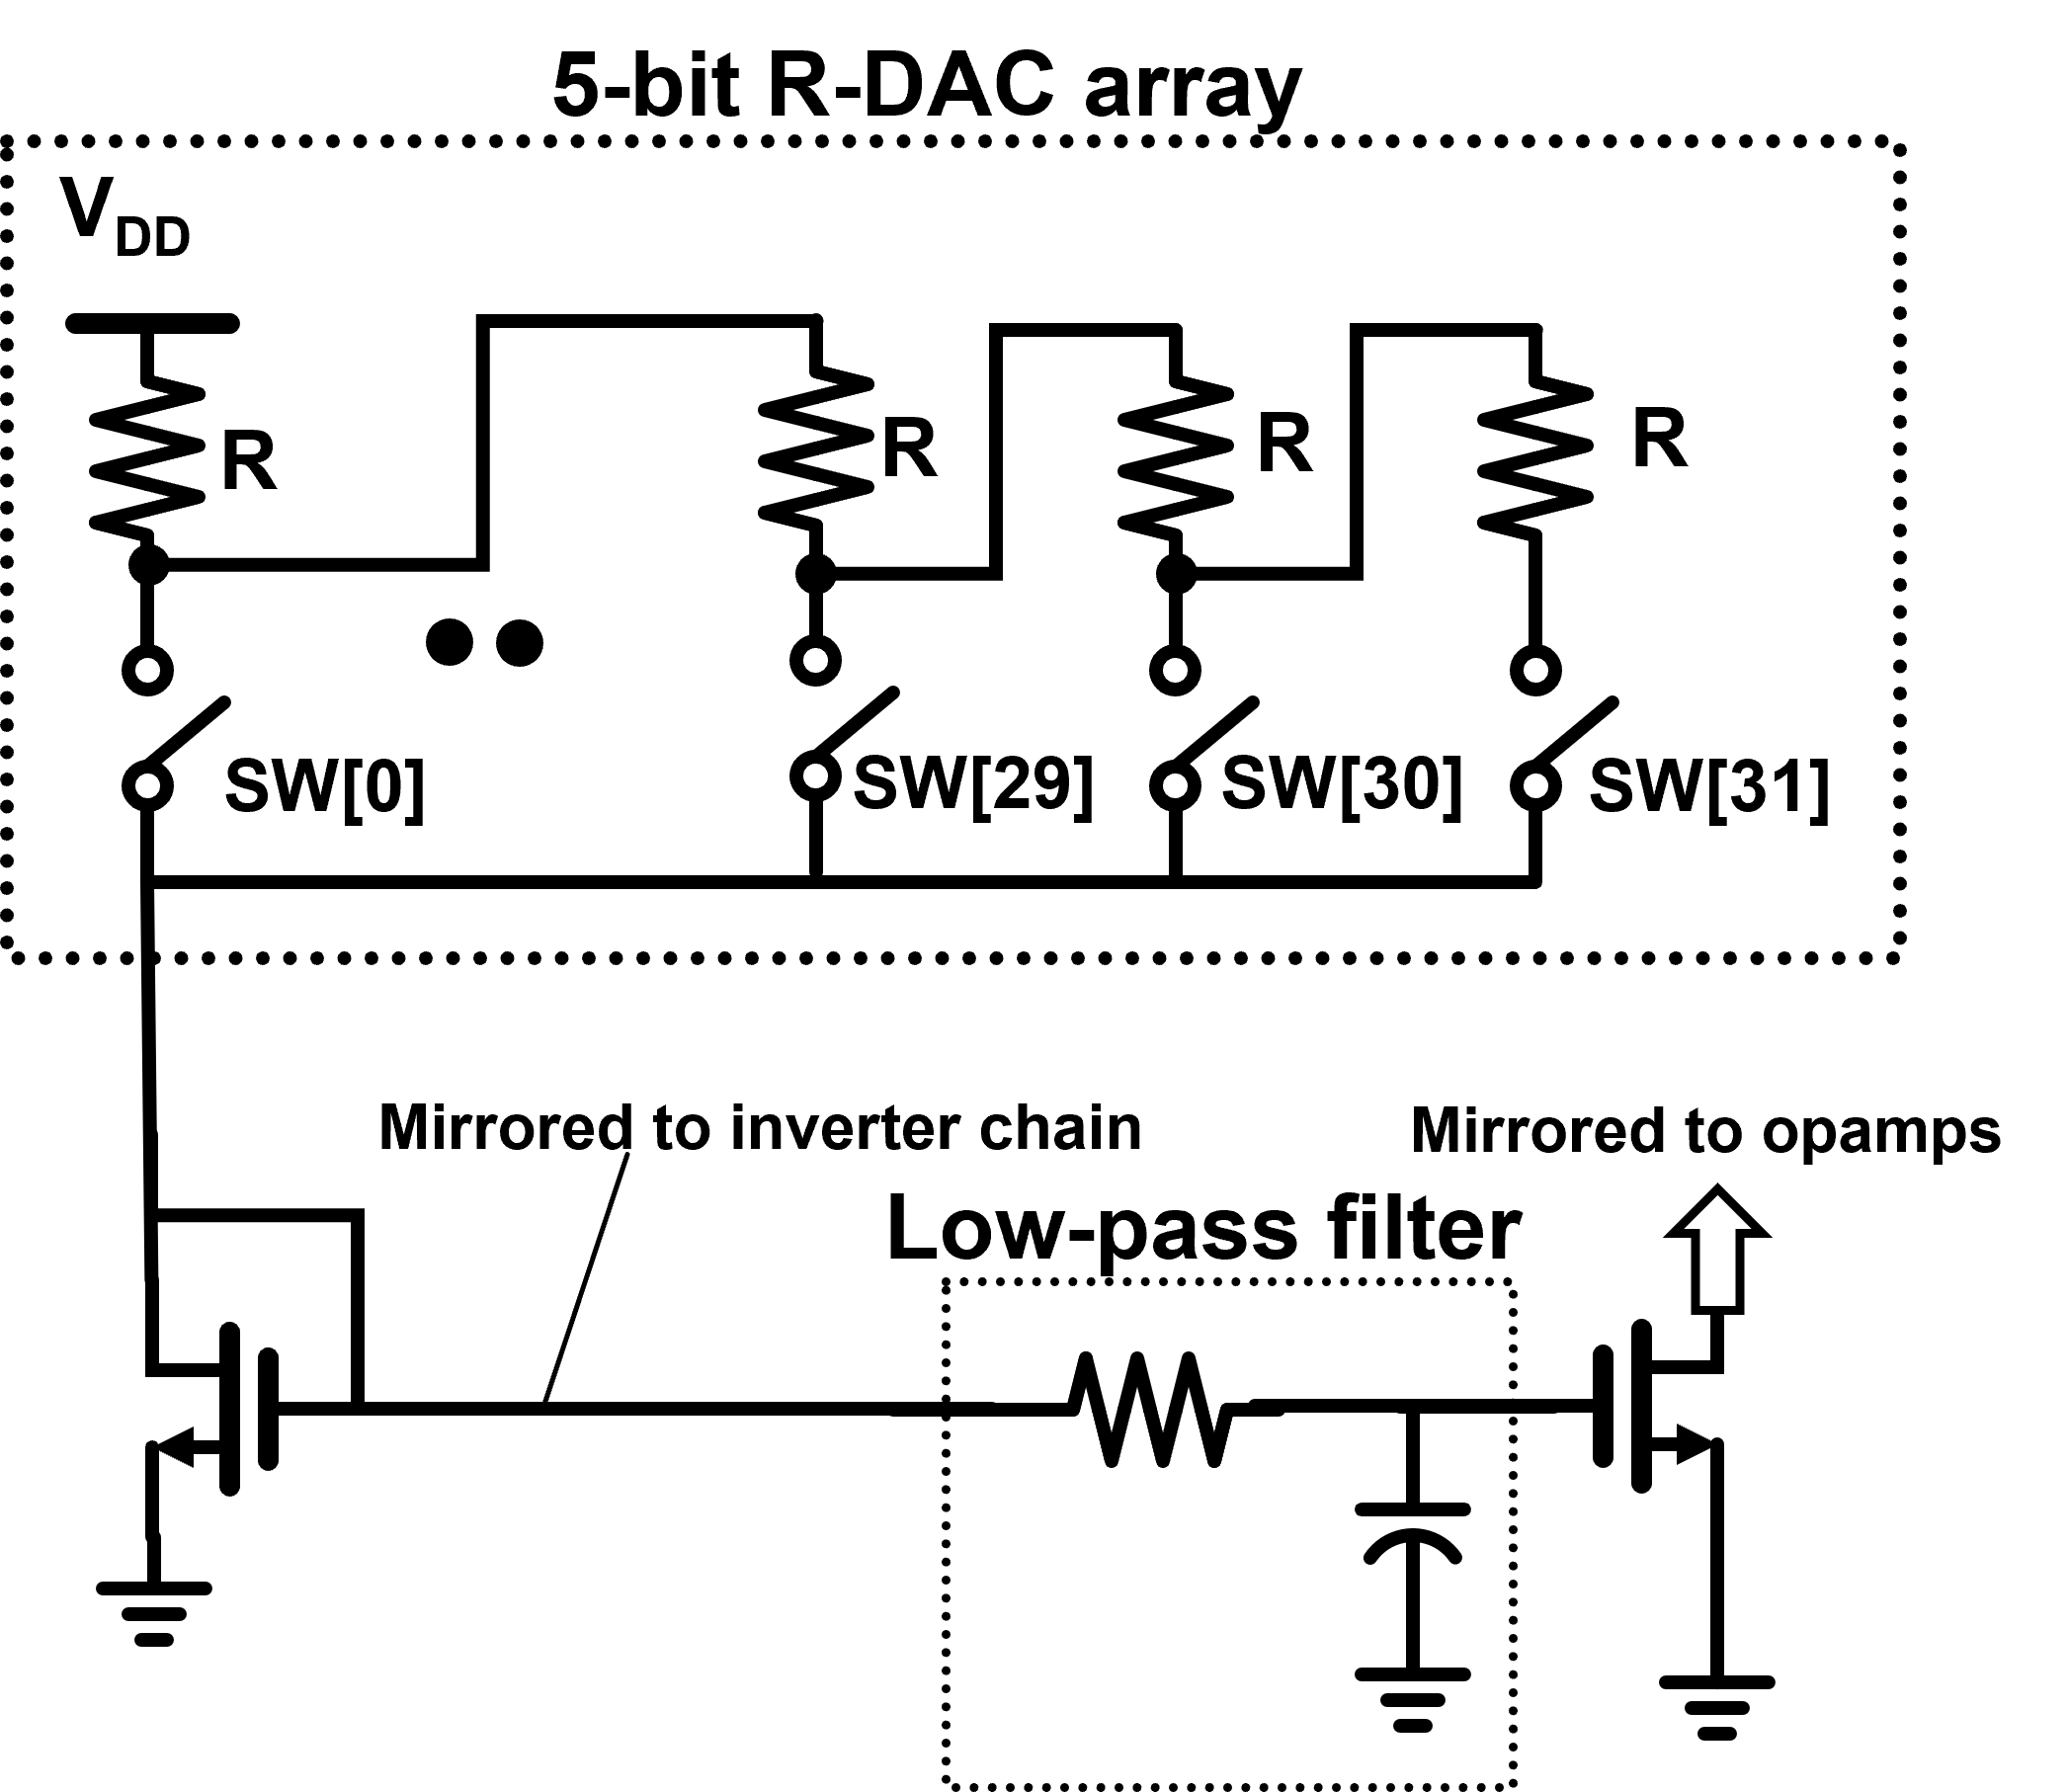
\includegraphics[width=0.5\textwidth]{figs/rdac.png}
  \caption{(a) 
}
\label{fig2}
\end{figure}
可変基準電流源を構成するR-DACの回路図を示す。電流値(IREF)は

$$I_{Ref} = \frac{V_{DD}}{R_{NMOS}+\sum R_{DAC}}$$

で決定されR-DACの抵抗値を制御することで電流制御を実現する。R-DACはone-hotのデジタル制御コード(SW[0:31])によって制御され、SW[31]がHighの時RDACは32Rとなり最大値を示し、SW[0]がHighの時抵抗値は最低でRDACはRを取る。TBCSでは抵抗DAC設計が最もクリティカルな要素となる。なぜならばR-DACの設計により生成電流の精度が必要十分か、そして抵抗ばらつき下でも目標電流値を生成できるかの2点を満たさなければいけないためである。

% Please add the following required packages to your document preamble:
% \usepackage{graphicx}
\begin{table}[]
\resizebox{0.5\textwidth}{!}{%
\begin{tabular}{|l|l|l|l|}
\hline
                           & 4-bit & 5-bit & 6-bit \\ \hline
current resolution{[}uA{]} & 5.3   & 1.3   & 0.3   \\ \hline
\end{tabular}%
}
\end{table}

まず式の通り抵抗DACの分解能は生成電流の分解能に直結する。R-DACを単位抵抗R=4kΩと一定で分解能を4,5,6 bitと変動させた際の電流分解能を表に示す。今回の設計値では4b DACでは5uAとステップは大きく設計にそぐわないものの、5bでは1.3uAと必要十分の精度が得られた。

\begin{figure}[!]
\centering
 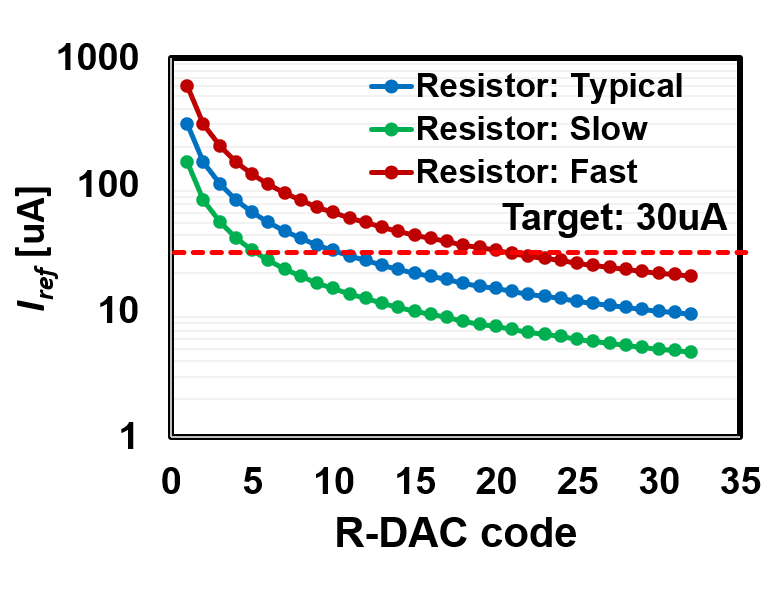
\includegraphics[width=0.5\textwidth]{figs/rdaccode.png}
  \caption{(a) 
}
\label{fig2}
\end{figure}

第2に抵抗のPVTばらつき下でも目標電流値にロックできるか確認しておく必要がある。図に抵抗のPVT におけるDACコードvs 生成電流をプロットした。今回目標とする30uAの電流生成はSlowからFast条件全てでカバーできることがわかる。もし抵抗ばらつきが大きくターゲットをカバーできないのならばR-DAC分化能を増やし抵抗可変範囲を広く取る必要がある。

また図に示すとおりTBCSは抵抗をスイッチングするため、抵抗切替時に不要なスプリアスがオペアンプに伝搬してしまう可能性がある。そのような不要成分を取り除くため受動素子によりローパスフィルタを構成しオペアンプへミラーするバイアスのスイッチング成分を除去している。

\subsection{Inverter}
最後に遅延素子について記述する。スケマを図に示す。

・ミスマッチは重要な要素。電流生成ばらつきに直結する一方で今回のように1uA分解能の電流生成TBCSでは影響が少ない。

・Nステージの遅延器の場合、単体遅延器のミスマッチより生じる遅延ばらつきをvarとするとvar*sqrt(N)と増加。

一方で信号成分(合計遅延)はN倍になるため1/sqrt(N)とばらつきは緩和される。

今回の設計ではσ=30ps程度であり、TDCの単位ステップが600psに対し十分小さくTBCSの電流値への影響は少ない。

・同様にジッタもDLL等では重要な要素だがTBCSでは重要ではない。ジッタは遅延量に比べ十分小さく、それでいてTBCSがロック後にはヒステリシスがあるため遅延器とTDCのジッタは生成電流に影響は与えない。


\section{Experiment and simulation analysis}
\begin{figure}[!]
\centering
 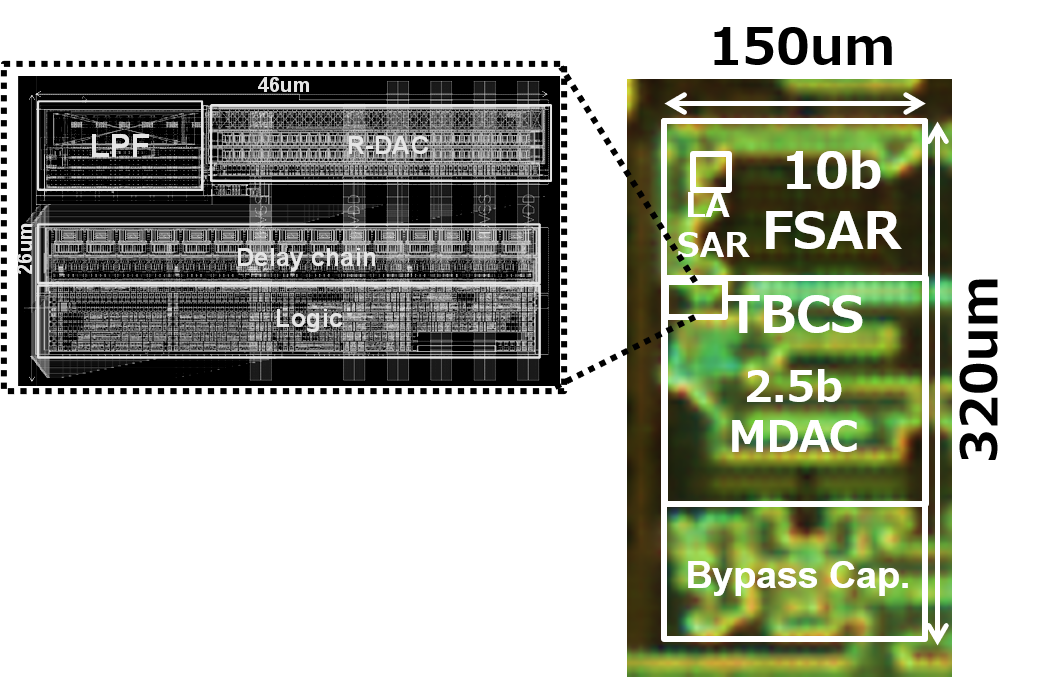
\includegraphics[width=0.5\textwidth]{figs/chip.png}
  \caption{(a) 
}
\label{fig2}
\end{figure}
\begin{figure}[!]
\centering
 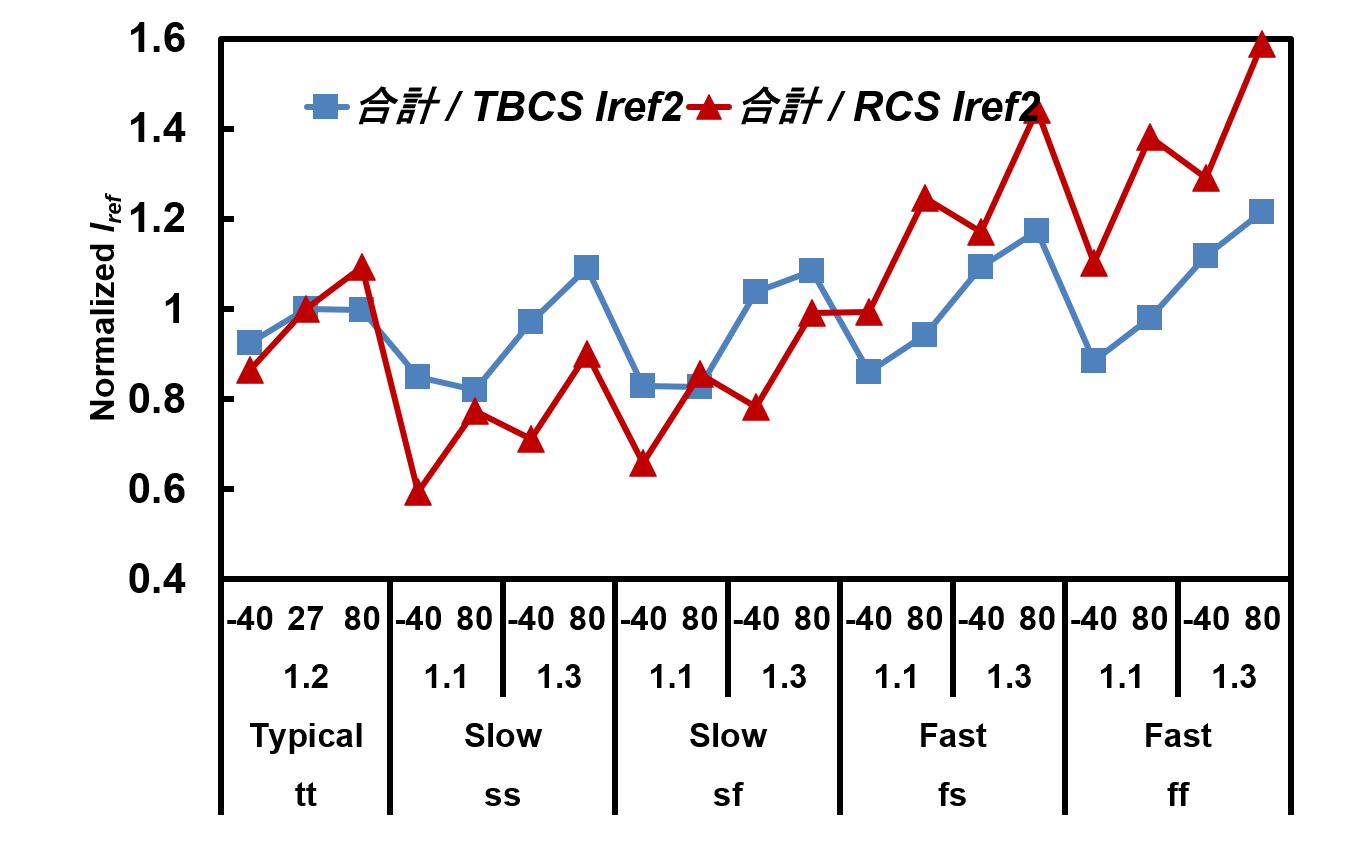
\includegraphics[width=0.5\textwidth]{figs/pvt.png}
  \caption{(a) 
}
\label{fig2}
\end{figure}
\begin{figure}[!]
\centering
 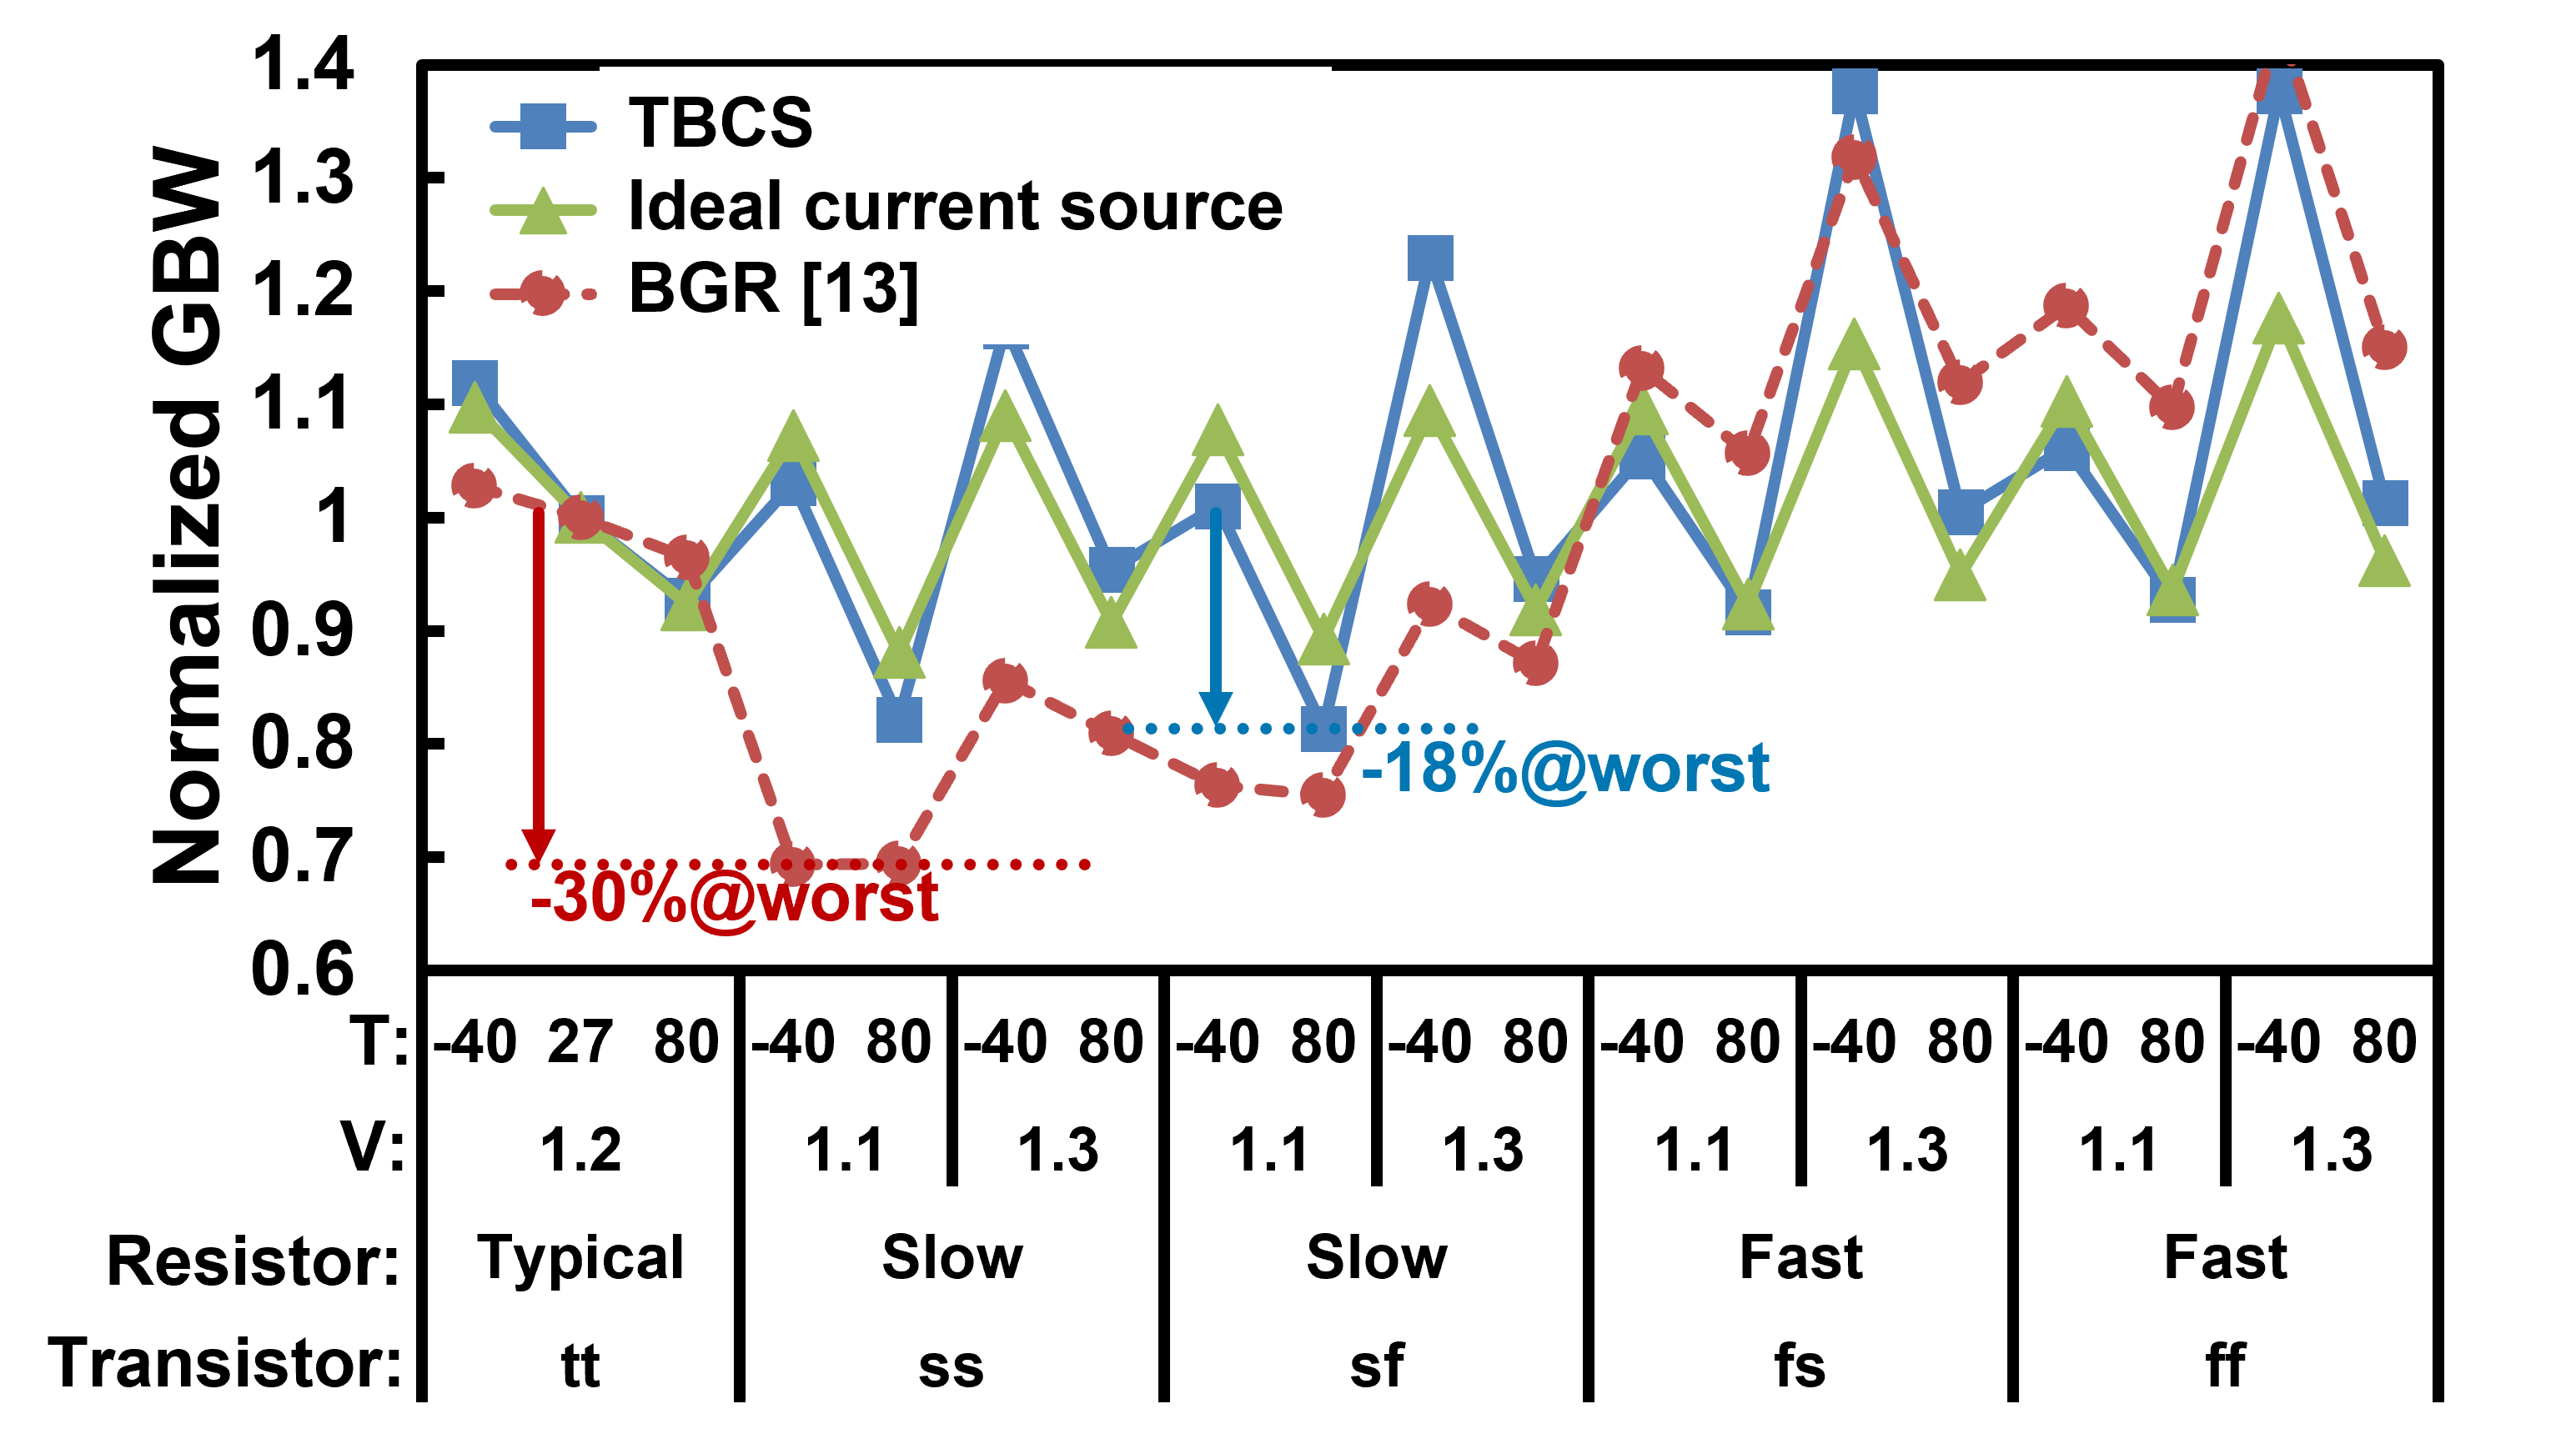
\includegraphics[width=0.5\textwidth]{figs/pvt_gbw.png}
  \caption{(a) 
}
\label{fig2}
\end{figure}
\begin{figure}[!]
\centering
 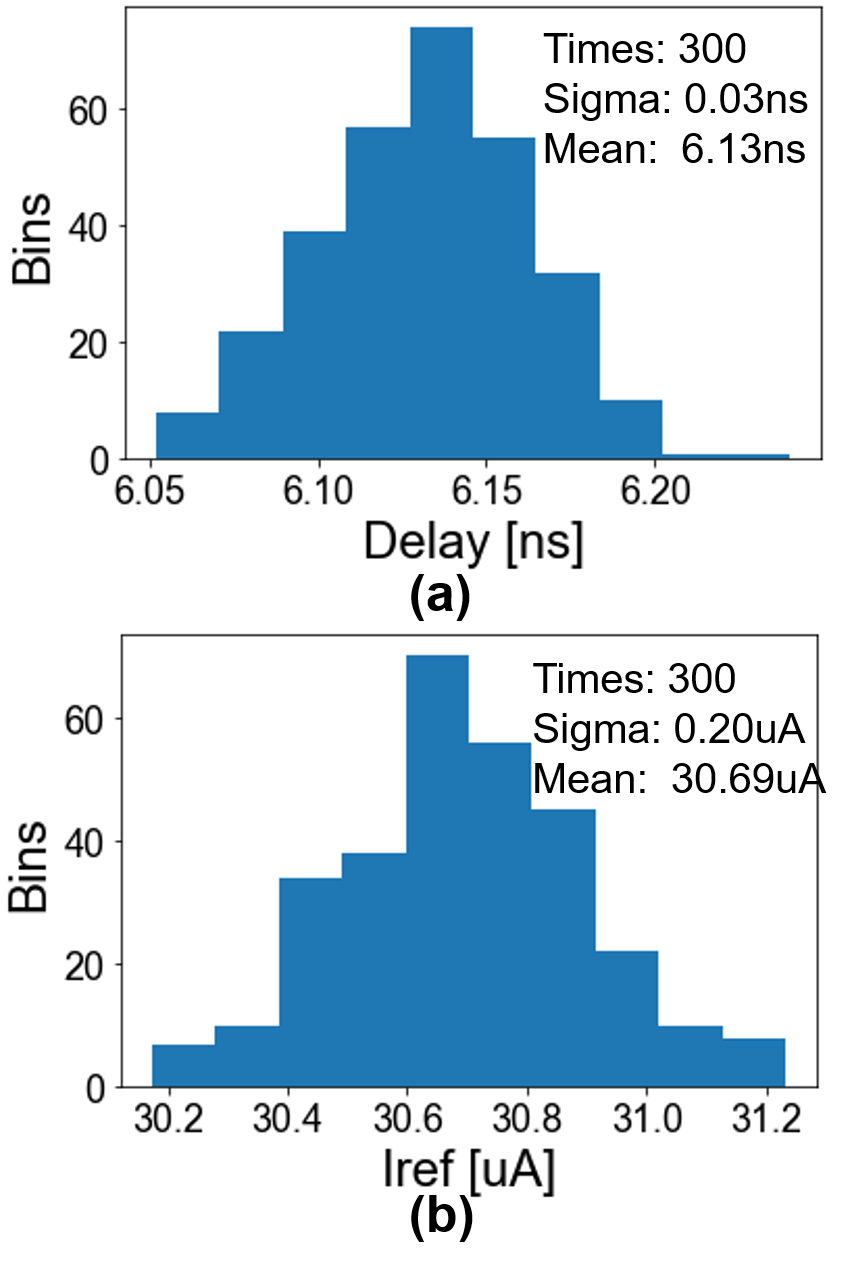
\includegraphics[width=0.4\textwidth]{figs/mc.png}
  \caption{(a) 
}
\label{fig2}
\end{figure}
## 1.1 従来電流源の電流特性

図 18 従来電流源の温度 vs 電流特性

まず比較のため従来電流源のPVTばらつきに対するシミュレーション結果を図 18に示す。ポリ抵抗及びバンドギャップ・リファレンスを用いた場合の回路を想定しており(図)、オペアンプは理想とした。ポリ抵抗はミスマッチはほとんどないものの、温度・トランジスタしきい値に対する感度が大きく、max min電流値は15uA離れている。ここで生じる問題としては:

**・SSLTLV(低温・減電)条件において電流値がtypに対し20%低下**

**・FF条件において電流値がtypの最大60%大きい**

ことである。前者はオペアンプ負荷のスイッチ抵抗増大等の効果もあり、オペアンプセトリング条件が最も厳しくなる条件で更に電流源値が20%も低下してしまうとセトリングを満足するのは厳しい。オペアンプ設計時にはSSLTLV条件のセトリングを満足するようにスルーレートを設定するため、typ含む他条件においてスルーレートは過剰気味になってしまい電力オーバーヘッドが生じてしまう。

またFF条件において電流値が大きく増加してしまうのもオペアンプ設計にもおいて問題が生じる可能性がある。FFではトランジスタしきい値降下はあるものの、IREFが増大してしまうとその分各トランジスタのVgsバイアス電圧を増加する必要がある。これはFF条件においてオペアンプの出力電圧範囲を狭めてしまう危険性をはらむ。オペアンプ電力を最小化するという観点ではSS条件では電流が多めになりFF条件では少なめになる(スイッチオン抵抗は低下するため)電流源が望ましい。

## 1.2 提案電流源の電流特性

図 19 提案電流源の温度 vs 電流特性

図 19に提案電流源を用いて温度対IREFをプロットした。28nmCMOSプロセスを用いてFFHTHV(125℃、1V)、TT(25℃、0.9V)、SSLTLV(-40℃、0.85V)にてスケマティックシミュレーションを実施している。これらのコーナー条件はトランジスタが最も速度が速いまたは遅い条件であり、他コーナー条件については後述する。入力しているクロック周波数は80MHzであり、その時に電流源は16.5uA出力するように遅延器を設計している。電流値はCount-up動作が終了しセトリングしたあとの値をプロットしている。

従来電流源との違いはまずPVT間で電流の差が少ないという点である。従来電流源の設計では抵抗値ばらつきによってmin-max電流値差が15uAもあったのに対し、提案では2uAとPVTばらつきを1/7程度に削減することができる。

また3章で述べた遅延器の電流-遅延特性について遅延量は後段インバータしきい値の関係上FFにおいて短くなりSSにおいて長くなる傾向を生じる。この効果も図 19から伺うことができる。SSにおいては遅延器にTTと同じ電流値を与えたとしても生成する遅延が長くなるため、80MHzで遅延ロックした時のIREFはTTよりも大きくなる。実際にシミュレーション結果からも1~2uAほどTTよりも大きい。これはオペアンプセトリングの厳しい条件においてオペアンプ速度を補填する方向に働くため好ましい。また同様にFFでは若干電流が減る方向に働くがオペアンプ速度要求が緩和されている条件のため問題ない。

図 20 全PVT条件vs電流特性(ミスマッチ込)

図 20に全PVT条件における出力IREF値をプロットした。レイアウト寄生抵抗+カップリング容量抽出シミュレーションにて求めている。またいくつか追加で非理想効果を追加してある:

**・遅延器のミスマッチ効果(3σ)**

**・クロックのDuty比(45%と55%の二種類)**

従来電流源では抵抗のミスマッチのみIREFに作用しており、そのようなミスマッチは小さく無視できた。しかし遅延器のトランジスタばらつきは無視できないほど大きく電流-遅延特性を変化させてしまう。モンテカルロシミュレーションでこのばらつきを見積もり、±3σのばらつきが生じた場合の電流値も同様にプロットした。FF、SFの高温条件において最悪値である12uA(typ値に対して25\%減)を記録するが、前述したとおりトランジスタが高速で動く条件のため電流が減少しても問題ない。同様に最高値もSS,SFの低温条件のみ発現するがオペアンプ速度を補填するため問題はない。

また入力クロックのデューティ比は45~55\%間でばらつく可能性がある。本電流源はデューティ比が変動すると入力クロック周波数が増減したのと同様の効果が現れてしまうが、45~55\%変動であれば大きな影響はない。

オペアンプのシミュレーションを行うときは単純に上記で得られたワースト・ベスト電流値を用いてPVTシミュレーションを行うのではなく、PVT毎のワースト・ベスト電流値で行うべきである。パラメータを入力する手間はかかるものの、SSでは速度補填効果等を実設計に組み込むことでオペアンプのオーバースペックを防止する。

## 1.3 電流源の入力周波数について

また本設計では入力クロック周波数は80MHzを念頭においている。WiFi受信機をアプリケーションとして考えているため他に動作モードとしては20MHz,40MHzが考えられ、そのような周波数の時は電流源コードは最低値に張り付いてしまう。オペアンプは電流が最低値でも問題なく動作するように検証を行った。例えば80MHzを念頭に設計した遅延器で40MHzにてロックしようとすると2倍長い遅延を作成する必要がある。張り付きが生じてしまう理由は可変電流源のレンジ不足であり、そのような遅延を生成するために必要な電流に設定できないためである。可変電流源のビット数を増やしより小さい電流も生成できるようにすれば問題はない。

図 21 遅延器の意図的発振を行う場合の回路図

また周波数を問わず一定電流を生成したいケースもあり、対応方法を記述する。もし入力周波数が整数倍の関係性がある場合(無線受信機用ADC等)、遅延器を意図的に複数回発振させることで一定電流を生成可能である。入力クロックが設計周波数の1/4(ex:20MHz)であることが既知でその情報をカウンタに入力できるとする。図 21のようにクロックがHighになると遅延器はクロックのエッジ情報を伝搬し、最終段遅延器は初段遅延器に帰還をかけ発振する(奇数段発振器と同等)。この図では遅延器が発振し4回目のエッジで位相比較を行う。この動作により遅延器は80MHzと同じ遅延量でロックするためIREFも同等になる。4回目のエッジが検出されたあとはENABLEを立ち下げることで発振も中止される。例えば遅延器のN段目出力を用いて位相比較を行うことでfractional周波数においても電流生成が可能である。カウンタを制御するための周波数情報は前もって入力する必要はあるが一般的にPLLはそのような情報を元に周波数を生成しているため情報を得るのは容易い。

\section{Conclusions}
To realize a fully adaptive noise scaling comparator, a VCO-based comparator with an eye-opening operation was introduced.  Even though the proposed VCO-based comparator was designed for a 13b ADC, this comparator can be used for further resolutions by carefully designing the jitter performance and the effective deadzone size. Moreover, since this comparator is mainly based on inverters and other simple logic cells, the comparator receives full benefits from process scaling. %Furthermore, the comparator characteristics can be analyzed with well-known knowledge of ring-oscillators. 

\bibliographystyle{IEEEbib}
\bibliography{main}


\begin{IEEEbiography}
[{
\includegraphics[width=1in,height=1.25in,clip,keepaspectratio]{bio/1.jpg}}]{Kentaro Yoshioka}
received his BS, MS, Ph.D degrees from Keio University, Japan. Currently, he is an Assistant Professor at Keio University. He worked with Toshiba during 2014-2021, developing circuitry for WiFi and LiDAR SoCs. During 2017-2018, he had been a visiting scholar at Stanford University, exploring efficient machine learning hardware and algorithms. 

Currently, Dr. Yoshioka serves as a technical program member of Symp. VLSI circuits conference. He was the recipient of ASP-DAC 2013 Special Feature Award, the A-SSCC 2012 Best Design Award, and 1st place winner of Kaggle 2020 Prostate Cancer Grade Assessment (PANDA) Challenge.
\end{IEEEbiography}

\end{document}
